\section{General overview}

To understand how eucalyptus is talked about, we first need to understand who is speaking about it. As such, we can first divide our dataset between two large groups of actors: persons and entities. In Figure \ref{fig:dist_author_year} we see the distribution of these two categories per year. While before 1860 the number of authors is low, documents about eucalyptus are mostly being published by authors. However, the number of "entities", rises after 1860. This is related to the general rise of articles talking about this new plant, which is thus mostly driven by entities.

\begin{figure}[H]
    \centering
    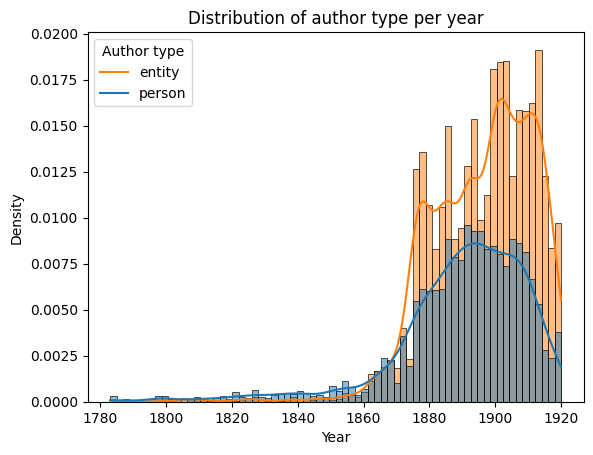
\includegraphics[width=0.5\linewidth]{Images/Figures/dist_author_year.png}
    \caption{Histogram depicting the distribution of documents per author type and per year.}
    \label{fig:dist_author_year}
\end{figure}

However, we can distinguish more than one type of entity that might be interested in publishing about eucalyptus. As such, we can divide these two categories (person and entity), into a typology of documents: monographs (which will mostly be published by "persons"), generalist press, specialized press, official press and directories. The distribution of authors and document type is shown in Figure \ref{fig:count_author_type}, and it clearly follows what we would expect: monographs are published by "persons" and the rest by "entities".

\begin{figure}[H]
    \centering
    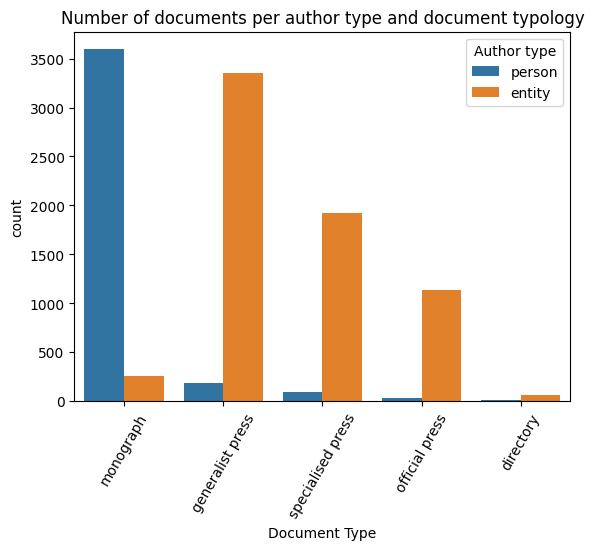
\includegraphics[width=0.45\linewidth]{Images/Figures/count_author_type.png}
    \caption{Bar plot displaying the number of documents per author and document type}
    \label{fig:count_author_type}
\end{figure}

It is then useful to look at the distributions of these different types of actors through time, to see if we discover certain patterns. Figure \ref{fig:dist_type_year} does show that the rise in the amount of documents is driven by the generalist press, while monographs and the specialized press follow a similar trajectory. While this could be an artifact of Gallica's corpus, we see in Figure \ref{fig:dist_Gallica_eucalyptus} that it should not be the case. While there is a gradual increase in the number of documents in Gallica's database until 1914, the sudden rise in documents related to eucalyptus in the 1870s is a different phenomenon. Moreover, the frequent ups and downs (i.e. the drop in the 1880s) in the amount of generalist documents compared to the other types do show a more fleeting usage of the word, possibly driven in the corpus by certain advertisement campaigns or punctual discussions on government policies. Finally, Figure \ref{fig:dist_type_year} does show an uptick in the official press starting from 1900, which is, as is further developed in Section \ref{sect:madagascar}, mostly related to the colonization of Madagascar.

\begin{figure}[H]
    \begin{minipage}{0.40\textwidth}
        \centering
        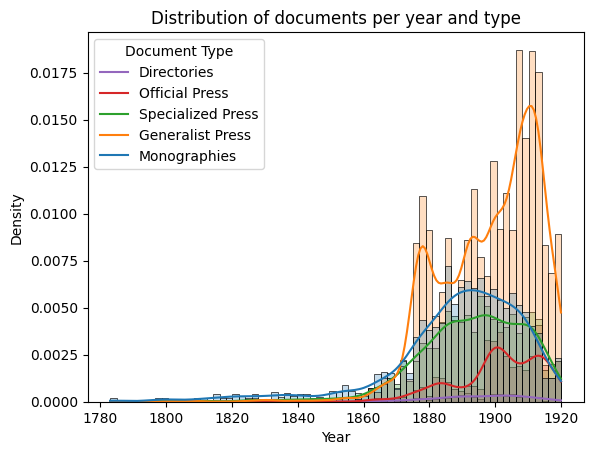
\includegraphics[width=\linewidth]{Images/Figures/dist_type_year.png}
        \caption{Histogram displaying the distribution of document types per year.}
        \label{fig:dist_type_year}
    \end{minipage}
    \hfill
    \begin{minipage}{0.48\textwidth}
        \centering
        \includegraphics[width=\linewidth]{Images/Figures/dist_Gallica_eucalyptus.png}
        \caption{Histogram comparing the yearly distributions of the eucalyptus corpus and the overall Gallica corpus.}
        \label{fig:dist_Gallica_eucalyptus}
    \end{minipage}
\end{figure}

We can also look at the distribution of documents per place of publication as in Figure \ref{fig:dist_place_year}. While the presence of Paris is expected, we do see a rise in documents published in the south of France starting from 1900, driven by the city of Lyon, which will be further developed in Section \ref{sec:lyon}. Moreover, the shape of the curve of documents published in Madagascar is quite similar to the official press, showing, as mentioned previously, the relationship between the two. The change in the 1860-70s is also visible, with an uptick of documents published in Paris, South of France and North Africa, while in the rest of Metropolitan France the rise is more steady. It probably comes from the fact that it is not a region of plantation and thus the number of documents does not share the same peak.

\begin{figure}[H]
    \centering
    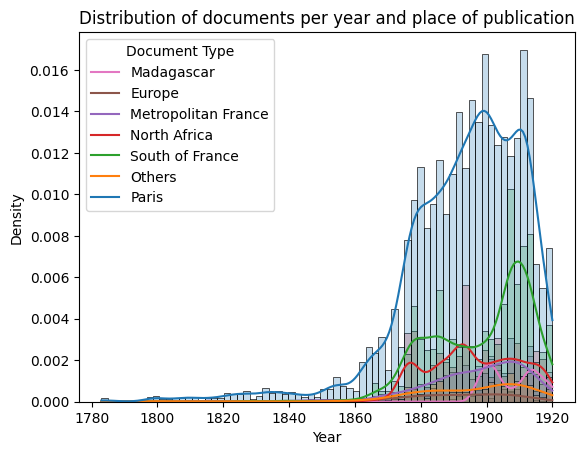
\includegraphics[width=0.45\linewidth]{Images/Figures/dist_place_year.png}
    \caption{Histogram displaying the yearly distribution of the publishing places of documents.}
    \label{fig:dist_place_year}
\end{figure}

Finally, to understand how eucalyptus is spoken about in the corpus, we can use topic modeling, as described in Section \ref{sec:met_topic_modeling}. Table \ref{fig:word_clouds} gives an overview of a few of the most relevant topics in the documents, while a full account can be found in Appendix \ref{app:topics}. The biggest one is topic 0, which talks about the place of origin of the tree. Given that it is a new plant in Europe at the time of study, the emphasis on Australia is not surprising. The second biggest topic however is about Algeria and North Africa. While it may be unexpected to see it so high, the tree was heavily planted in the region after 1970. The fact that "Trottier", a key figure in the implementation of eucalyptus plantations in Algeria, appears in the topic shows the relationship between the region and the tree and why it is a key topic in the corpus. Finally, topics 3 and 9 show a key reason for the plantation of eucalyptus. Indeed, the tree was used as an answer to drain marshes, both to fight against malaria and to transform them into arable land, more suitable for European settlers \footnote{\cite[6]{davin-mortier_leucalyptus_2026}}. In the end, the model found 135 different topics, with a heavy tailed distribution (Figure \ref{fig:dist_context_topic}), emphasizing the importance of the larger topics, but with smaller ones still having a good number of contexts.

%TODO: CHANGE CITATION TO Doughty, The Eucalyptus: A Natural and Commercial History of the Gum Tree, 36.

\begin{figure}[H]
    \begin{minipage}{0.42\textwidth}
        \centering
        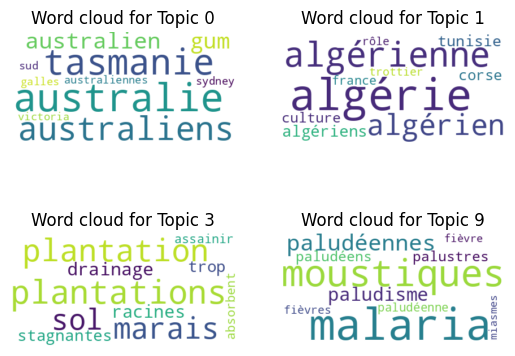
\includegraphics[width=\linewidth]{Images/Figures/word_clouds.png}
        \caption{Word clouds displaying the words most associated with topics 0, 1, 3 and 9.}
        \label{fig:word_clouds}
    \end{minipage}
    \hfill
    \begin{minipage}{0.42\textwidth}
        \centering
        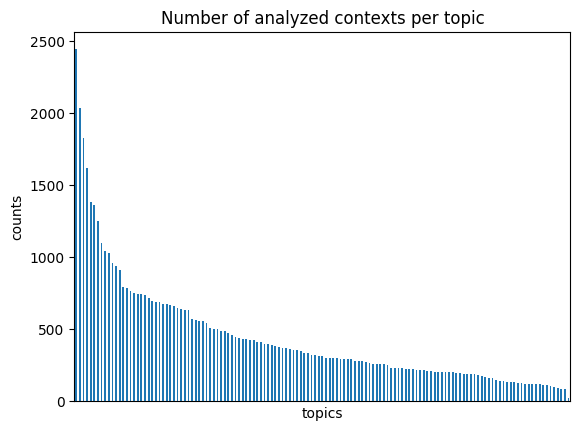
\includegraphics[width=\linewidth]{Images/Figures/dist_context_topic.png}
        \caption{Histogram displaying the distribution of the number of contexts per topic.}
        \label{fig:dist_context_topic}
    \end{minipage}
\end{figure}

Given their amount, we can group them into meta-topics, and analyze their distribution within the typology previously discussed. The result is presented on Figure \ref{fig:dist_metatopics_type_norm}, showing the distribution of each meta-topic within each category. The results do show a prevalence for Institutional topics within the official press, more scholarly topics (medicine and botanical and historically related) in monographs and specialized press and a bigger amount of "Others" in the generalist press. We can also look more at the way the medicine-related topics are distributed. We really do see this separation between monographs and the specialized press against the generalist press, whereas the first group do have a good amount of contexts related to the chemical properties of the plant and its medicinal and medication uses, the generalist press only covers medicine and medication (and in a smaller amount), probably related to advertisements of such products, as will be seen further in the analysis.

\begin{figure}[H]
    \begin{minipage}{0.48\textwidth}
        \centering
        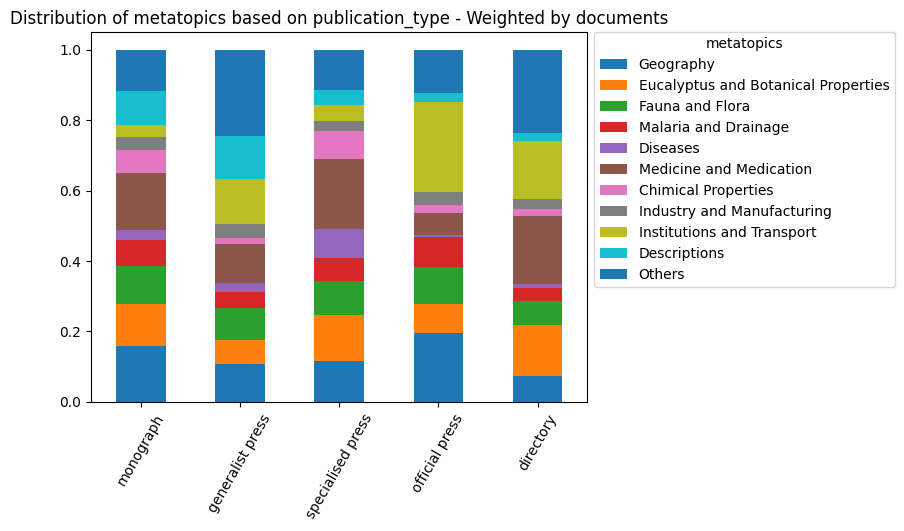
\includegraphics[width=\linewidth]{Images/Figures/dist_metatopics_type_norm.png}
        \caption{Bar plot displaying the distribution of meta-topics within document types.}
        \label{fig:dist_metatopics_type_norm}
    \end{minipage}
    \hfill
    \begin{minipage}{0.48\textwidth}
        \centering
        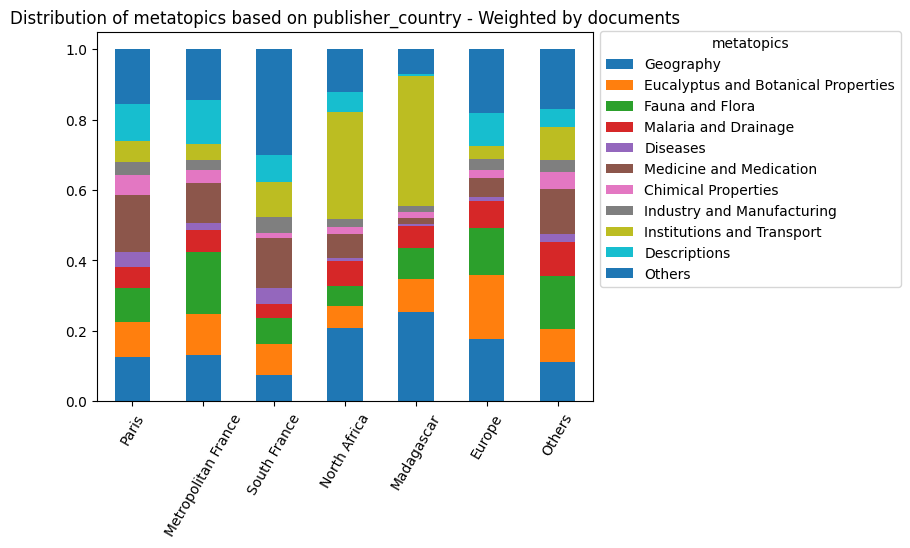
\includegraphics[width=\linewidth]{Images/Figures/dist_metatopics_place.png}
        \caption{Bar plot displaying the distribution of meta-topics within publishing regions.}
        \label{fig:dist_metatopics_place}
    \end{minipage}
\end{figure}

We can also look at the meta-topic distribution within place of publication (Figure \ref{fig:dist_metatopics_place}). We see similar distributions between Paris, Metropolitan France and Others, while topics in North Africa and Madagascar are clearly skewed towards Institutional ones. It is interesting to note that both colonized regions appear with similar distributions, as it shows that the tree does appear in similar way in the context of colonization, notably through institutional means. At last, we can notice that the topic "Malaria and Drainage" does appear consistently around 5\% in each region. Historically one of the main drivers of eucalyptus plantation, while it does not seem to be the main driver of discussion in published documents, it is still consistently in the same proportions in each region, showing that it remains a key reason for plantation and thus in the discussion around the tree. The fact that it appears only around 5\% is thus probably linked with the number of generalist press, which will likely talk less about this subject.

After this overview of the results, three case studies will be analyzed in depth in this section, based on the interesting results from the overall data. First, we will look at the rise in documents in Lyon starting from the 20th century, then at the publications from Madagascar in the same time period, and finally at the evolution of the documents related to the drainage of marshes and the fight against malaria.

\section{Lyon between 1900 and 1920}
\label{sec:lyon}

In order to understand the importance of eucalyptus in Lyon during this time period, we first need to better understand what makes it a good case study.  Looking at the distribution of documents per year and place of publication in Figure \ref{fig:dist_place_year}, we see a clear rise in the documents published in the south of France starting from 1900. When investigating closer, we see that after 1900, 67\% of documents published in the south of France were from Lyon, whereas the proportion before 1900 is only of 20\%. This change shows that a phenomenon happened within the documents published in the region.


We can then look at which documents influence this rise. As Figure \ref{fig:dist_lyon_type_year} shows, it is clearly pushed by a rise in the generalist press, led by the journal "Le Progrès", which accounts for 1187 of the total 1458 documents published in Lyon during this time frame. We can discard the hypothesis of the implementation of a new journal, as, according to Gallica, "Le Progrès"'s first publication was in 1859 and the journal has been published daily since then. Thus, as eucalyptus appearances only start from 1900, this is clearly something new happening in this particular journal.

\begin{figure}[H]
    \begin{minipage}{0.48\textwidth}
        \centering
        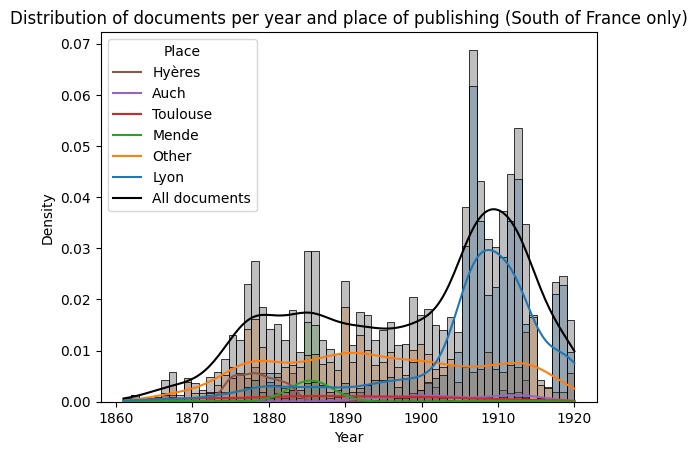
\includegraphics[width=\linewidth]{Images/Figures/dist_s_france_year.png}
        \caption{Histogram displaying the yearly distribution of documents per cities in Southern France.}
        \label{fig:dist_s_france_year}
    \end{minipage}
    \hfill
    \begin{minipage}{0.43\textwidth}
        \centering
        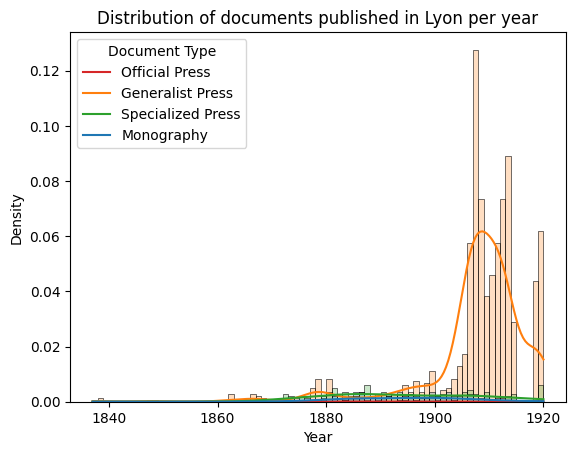
\includegraphics[width=\linewidth]{Images/Figures/dist_lyon_type_year.png}
        \caption{Histogram displaying the yearly distribution of documents published in Lyon per document type.}
        \label{fig:dist_lyon_type_year}
    \end{minipage}
\end{figure}

To understand what it is talking about, we can look at the topic distribution within the documents published in Lyon, as shown in Figure \ref{fig:dist_topics_lyon}. We clearly see that the meta-topic "Others" is in 40\% of documents published in the city. By looking more in-depth at the topic distribution within "Others", we find that 50\% of those is the topic 46. It speaks about pharmaceutical entities, such as "elixir" or "vermifuge", while also mentioning some units of measure as "litre" or "kilo". Looking at it without context, the words probably indicate a topic linked with a specific pharmaceutical advert. And indeed, we do find such and advert in several issues of "Le Progrès", as seen in Figure \ref{fig:img_le_progres_1906}.

\begin{figure}[H]
    \begin{minipage}{0.55\textwidth}
        \centering
        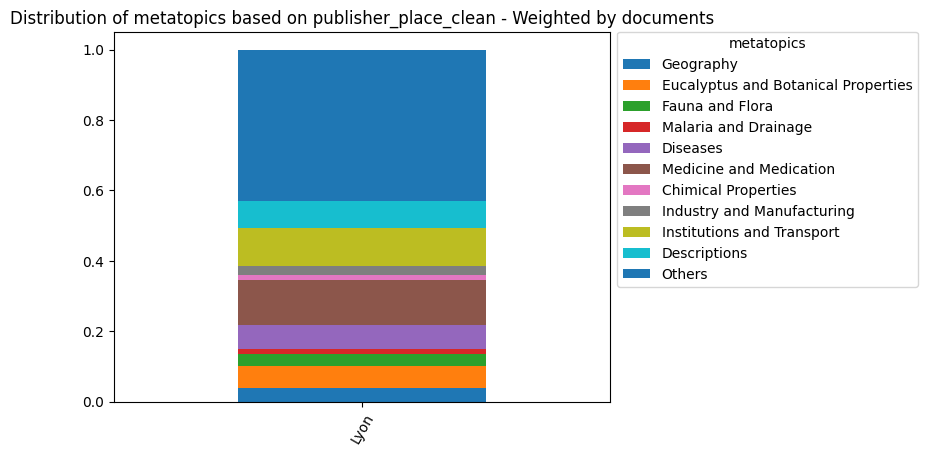
\includegraphics[width=\linewidth]{Images/Figures/dist_topics_lyon.png}
        \caption{Bar plot displaying the distribution of meta-topics within Lyon.}
        \label{fig:dist_topics_lyon}
    \end{minipage}
    \hfill
    \begin{minipage}{0.40\textwidth}
        \centering
        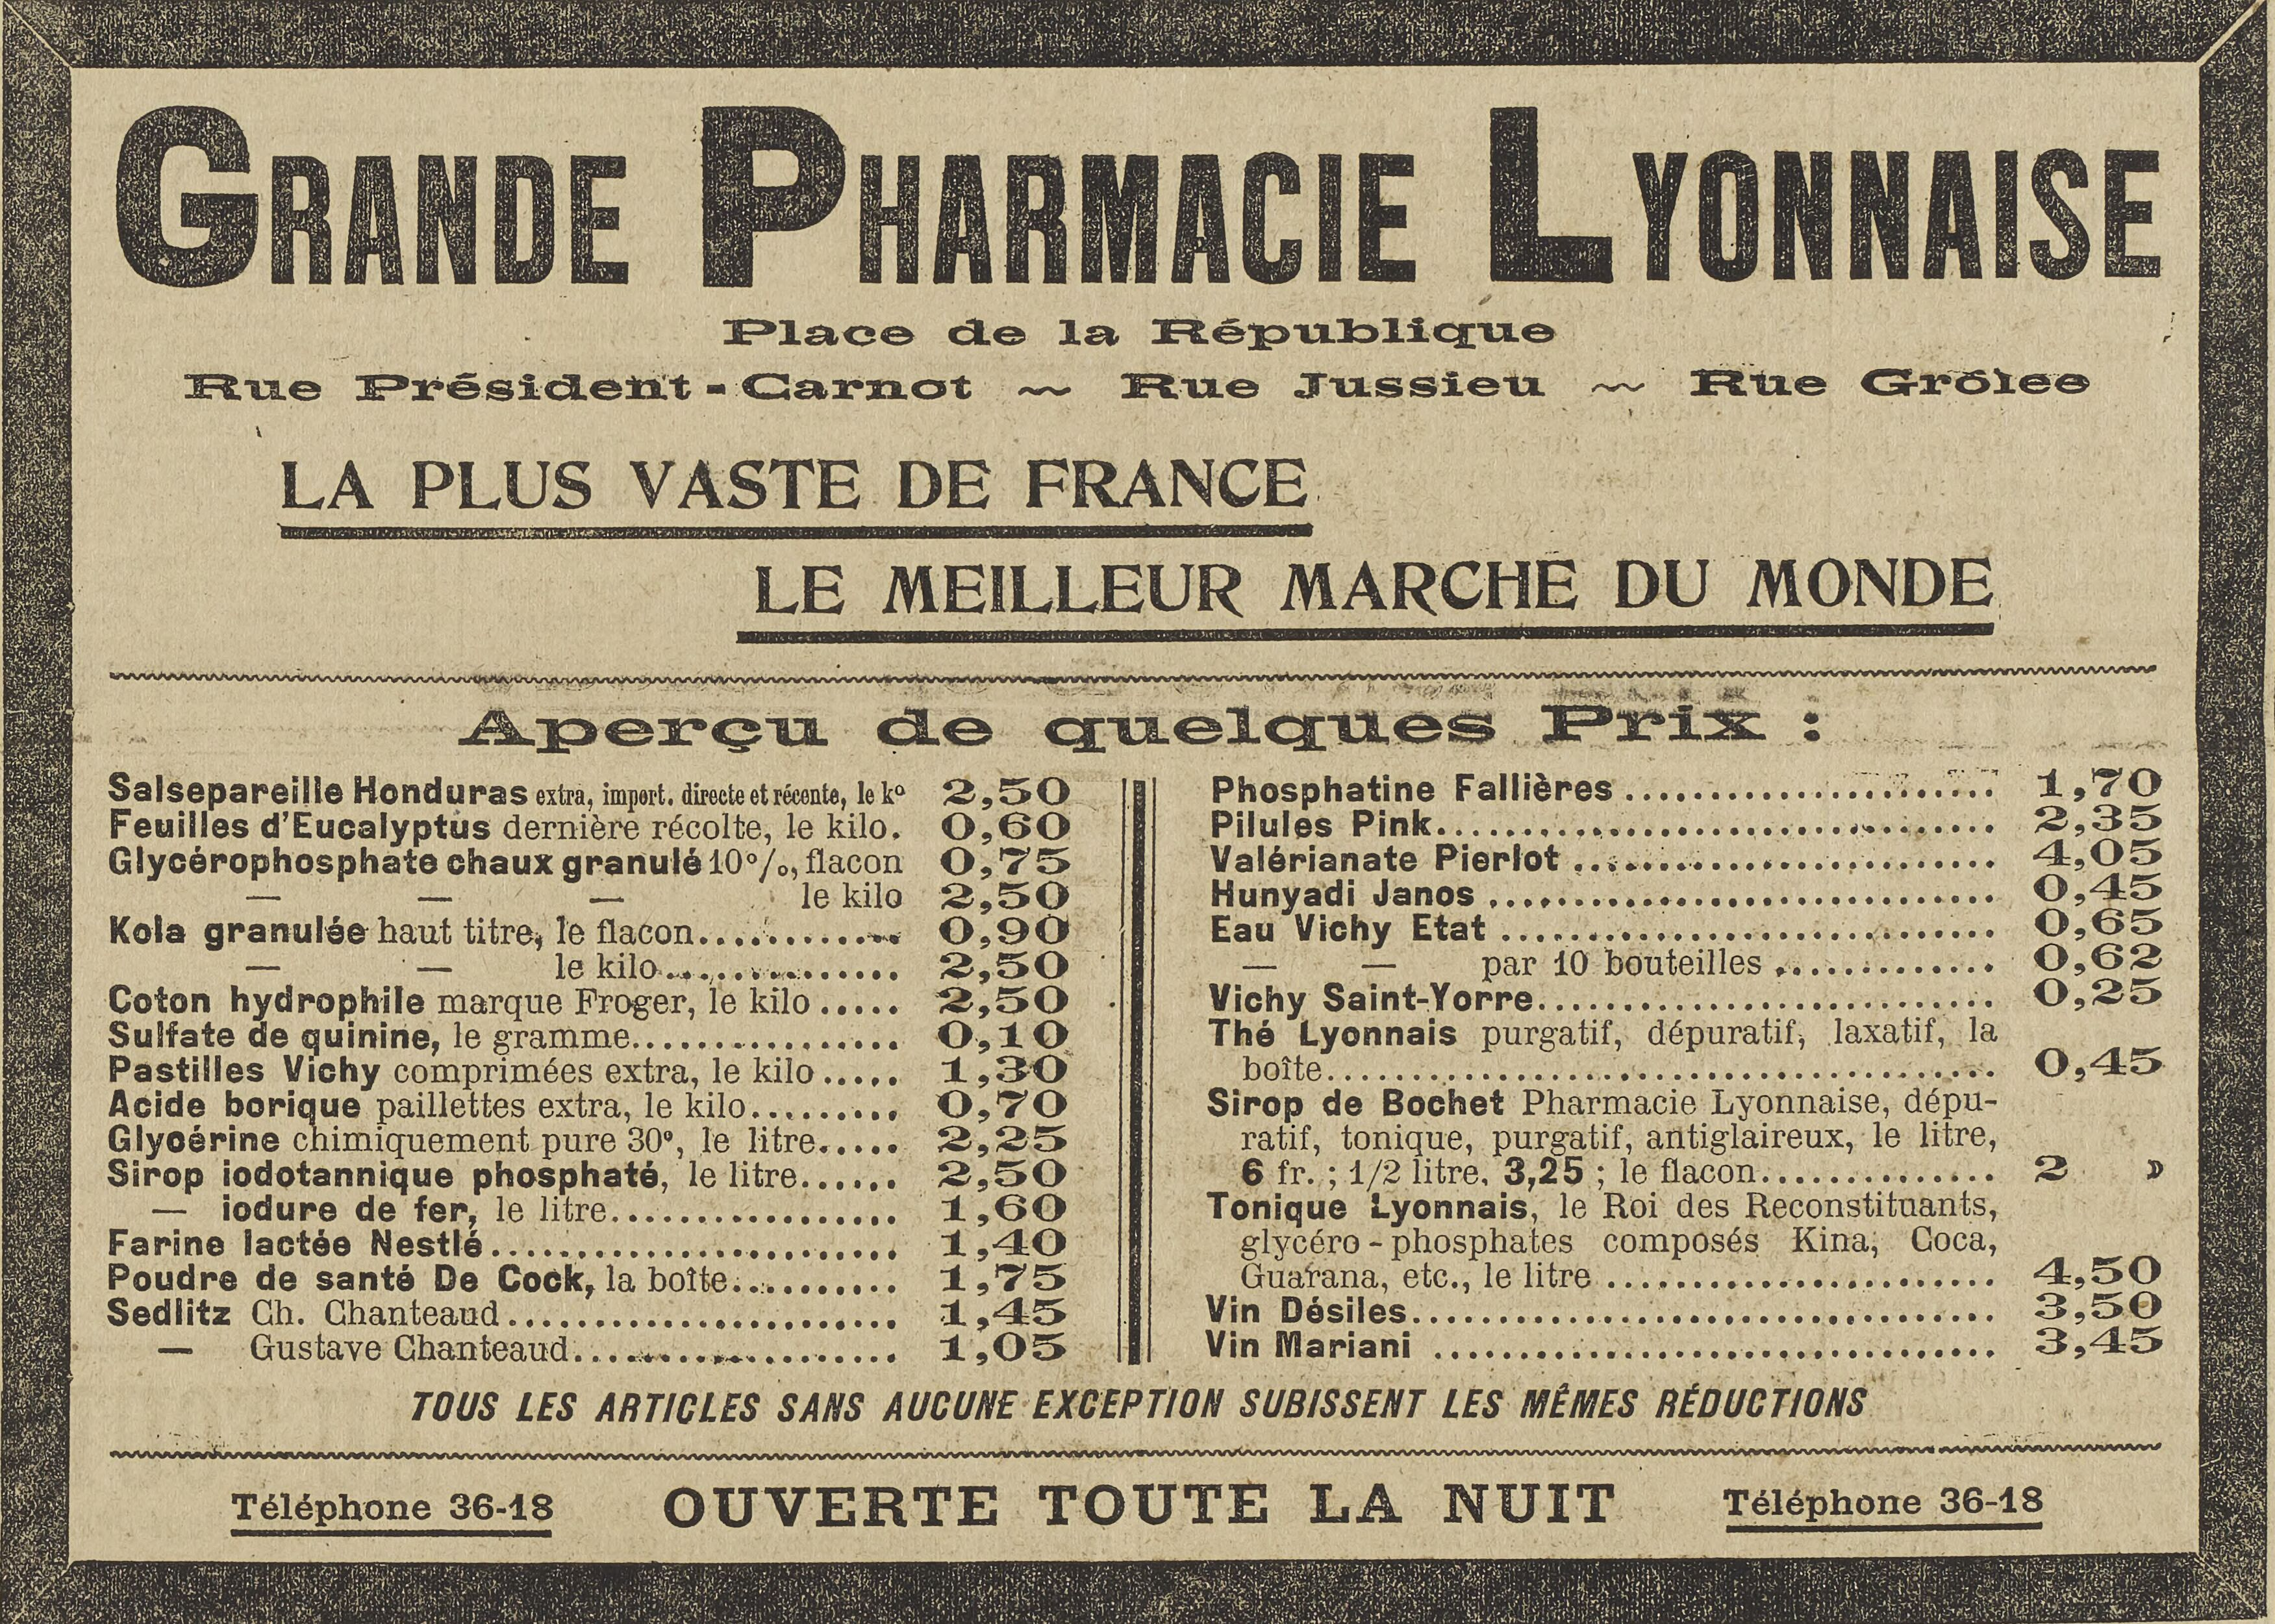
\includegraphics[width=\linewidth]{Images/Journals/Le_Progrès_1906.jpg}
        \caption[Advert for the "Grande Pharmacie Lyonnaise" in "Le Progrès"]{Advert for the "Grande Pharmacie Lyonnaise"\protect\footnotemark}
        \label{fig:img_le_progres_1906}
    \end{minipage}
\end{figure}
\footnotetext{\cite{noauthor_progres_1906}}


To see if such topics are indeed what drives this spike in Lyon, we can look at the topics over time. Topics 46 and 88 represent respectively ~25\% and ~8\% of all topics in Lyon and both are linked with advertisement. The first, as seen in Figure \ref{fig:img_le_progres_1906} with the "Grande Pharmacie Lyonnaise", and the second with an advert of an eucalyptus and honey based medicament against tuberculosis ("War against Tuberculosis") \footnote{\cite{noauthor_progres_1907}}, which explains why a word such as "war" is linked with more medical terms such as "tuberculosis" or "pectoral". By looking at their frequency over time (Figure \ref{fig:dist_topics_time_lyon}, we do see that they are highly focused in certain time-frames: 1908-1913 for topic 46 and 1904-1906 for topic 88. These match with the rise of documents mentioning "eucalyptus" published in Lyon, thus showing that advertisements are a key medium through which eucalyptus is talked about. Moreover, it is also interesting to note the environment in which the tree is used within these advertisements. Both are linked with the pharmaceutical and medicine industry, thus already showing its place as a plant with medicinal virtues in the collective mindset.

\begin{figure}[H]
    \centering
    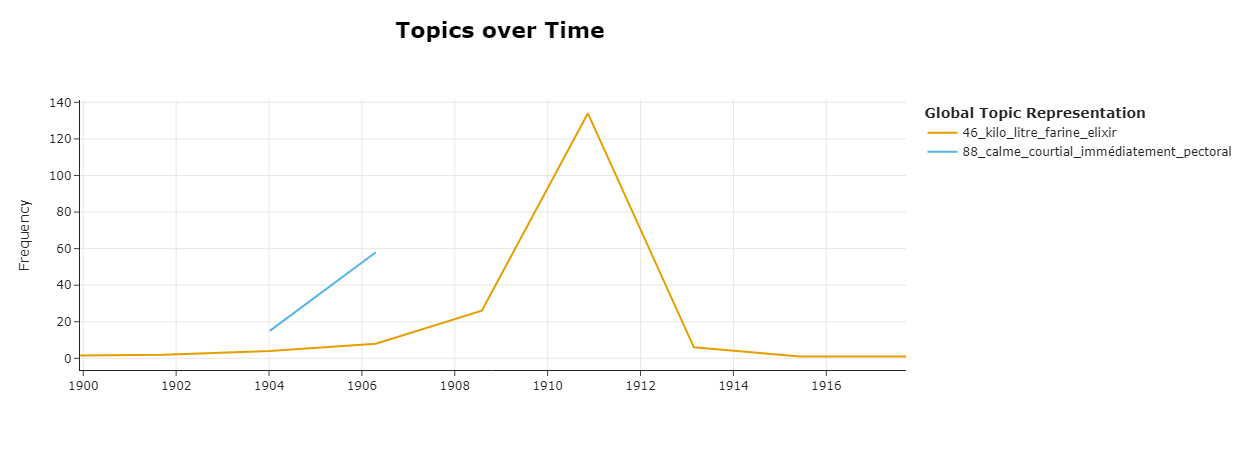
\includegraphics[width=\linewidth]{Images/Figures/dist_topics_time_lyon.png}
    \caption{Line plot displaying the yearly frequency of topics 46 and 88 in the corpus.}
    \label{fig:dist_topics_time_lyon}
\end{figure}

To conclude, while Lyon is a clear case study of publicity in relation with eucalyptus, this phenomenon appears throughout the corpus, and is often captured in specific "advertisement" topics. These are often local to specific cities and capture advertisements that appear throughout several documents. Topics 46 and 88 for example, appear overwhelmingly in Lyon only, with respectively 78\% and 62\% of the documents related to those topics coming from there. Thus, other similar "advertisement" topics can be found, such as topic 72 with 52\% of it's documents published from "Mende" (who only represents 0.6\% of the total number of documents). Such appearances of advertisements should not be overlooked when analyzing the discourse around eucalyptus, as it shows us what is the appeal of the tree. Indeed, advertisements aim to sell products and as such will use (or try to build) a shared imagery on what the plant is and what its qualities are. Thus, as advertisements are mostly linked with medicinal properties and usages, these are clues to understand what the general population thinks, or is invited to think, of the tree.


\section{Madagascar and the official press}
\label{sect:madagascar}

While Lyon showed the importance of the adverts in the number of documents related to eucalyptus, Madagascar shows the importance of the official instances, and how this plant seems to be used as a tool for land planning. Indeed, it was in 1896 that French troops invaded and took control of the island \footnote{\cite[79]{sanchez_letat_2018}}, and this colonization process is seen in the corpus, as the first instance of the "Journal officiel de Madagascar et dépendences" in the corpus dates from 1897, and until 1920 it appears 459 times (around 20 instances per year for a journal published around once or twice a week, based on Gallica's data). Moreover, this journal accounts for 86\% of all documents published in Madagascar within the corpus, showing both the importance of the official documents in relation with eucalyptus, and seemingly the lack of a generalist francophone press at the early stages of the colonization process.

Having established that eucalyptus were talked about in Madagascar's official documents, it is important to learn how it was talked about and for which purposes it was used. We can thus look at the distribution of meta-topics within the documents published in the island (Figure \ref{fig:dist_topics_madag}). It shows us that close to 40\% of the topics mentioned in the area belong to "Institutions and Transport", a bit more than 20\% to "Geography", while meta-topics related to technical and scientific skill ("Medicine", "Chemical Properties" and "Industry and Manufacturing") are almost negligible. 


\begin{figure}[H]
    \centering
    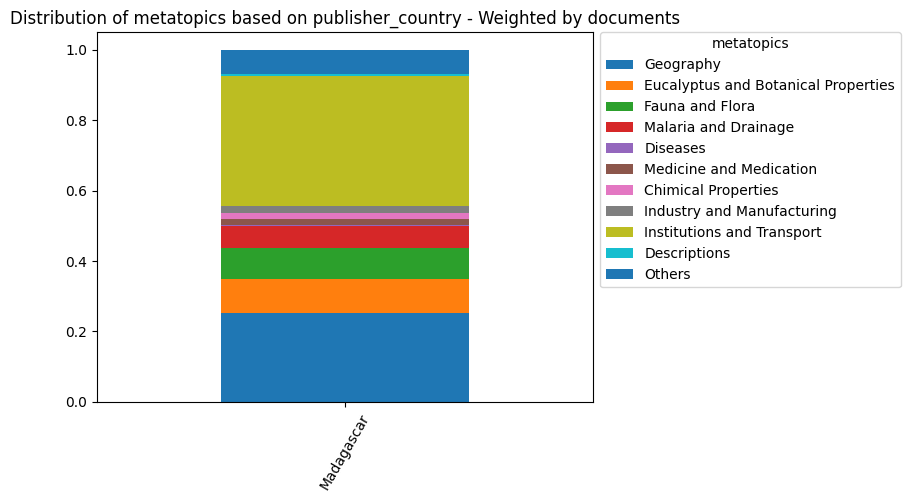
\includegraphics[width=0.55\linewidth]{Images/Figures/dist_topics_madag.png}
    \caption{Bar plot displaying the distribution of meta-topics within
Madagascar.}
    \label{fig:dist_topics_madag}
\end{figure}

Based on the previous distribution, it is important to focus on the topics belonging to "Geography" and "Institutions". Looking at both, topic 43 represents 80\% of all the "Geography" meta-topic (and $\sim$30\% in total), while topic 80 represents close to 75\% of all "Institutions" meta-topic ($\sim$23\% in total). This shows that the tree appears in rather uniform contexts within the island's publications. It is interesting to note that the third biggest topic is topic 3. While its distribution within Madagascar and the rest of the corpus is not that different ($\sim$5\%), it shows that drainage is still one of the main roles fulfilled by eucalyptus in Madagascar. Moreover, there is close to no document co-occurrence between topic 3 and topics 43 and 80 (only 2 and 3 documents respectively), showing that the issue of soil drainage is spoken about in different contexts than issues related to the institutions (which often co-occurs with the geography topic).

Looking at the words inside the biggest topics, number 43 represents Madagascar ("Fianarantsoa", "Malgaches"), its regional administration ("district", "canton") and administrative terms, probably related with its colonization history ("réquisition", "né(e)"). As such, it does make sense that it appears as the biggest topic in the island's publications. Topic 80 on the other hand has words in the lexical field of decision making and administrative settings ("déclaré", "demandé", "propriétaire"). Knowing that most of the documents published on the island are from the official press, these words make sense. However, it is interesting to note other words in the topic, such as "patates" or "manioc", showing that eucalyptus appears in the same context as food production. 
To better understand it, we can look at examples of documents in which topic 80 appears, such as in Figure \ref{fig:img_Journal_Madagascar_1904}. This document describes the requisition of a property close to Tamatave, which is then received by a local administrator. Eucalyptus are thus present in the description of the property's terrain, as well as the above-mentioned "patates" and "manioc". This example, far from being isolated, shows that the tree is already quite established in the island and is discussed in the same way as other food related plants. 

\begin{figure}[H]
    \centering
    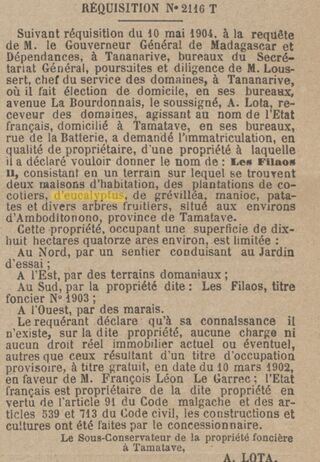
\includegraphics[width=5cm]{Images/Journals/Journal_Officiel_Madagascar_1904.jpg}
    \caption[Requisition of a land parcel close to Tamatave]{Requisition of a land parcel close to Tamatave\protect\footnotemark}
    \label{fig:img_Journal_Madagascar_1904}
\end{figure}

\footnotetext{\cite{madagascar_journal_1904}}

By looking at the amount of contexts by year, related to the three topics discussed above (3, 43 and 80) by year (Figure \ref{fig:dist_topics_year_madag}), we see that topic 3 is quite infrequent but relatively stable. However, topics 43 and 80 clearly rise starting from 1910, but then drop at start of the war. This probably shows one of the reasons why eucalyptus are being planted in Madagascar, but also the amount of properties which already have the tree in their descriptions.

\begin{figure}[H]
    \centering
    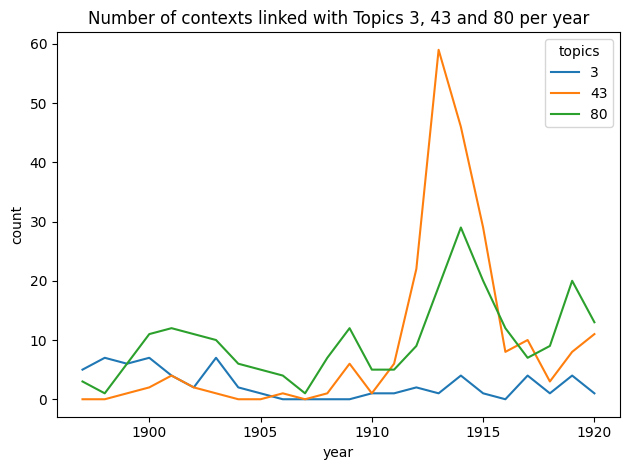
\includegraphics[width=0.5\linewidth]{Images/Figures/dist_topics_year_madag.png}
    \caption{Line plot displaying the yearly number of contexts in Madagascar  linked with topics 3, 43 and 80.}
    \label{fig:dist_topics_year_madag}
\end{figure}

In conclusion, we see a region that immediately after the French conquest starts producing literature that mentions eucalyptus. These documents are heavily linked with institutions, showing that there is not yet a solid French presence on the island, as there is not really any generalist press for local settlers, as can be seen in Algeria. Here, most documents concern administrative regions and the requisition of properties by the settlers. The tree is here often mentioned alongside plants related to the food industry in terrain descriptions, showing that it is already present in the island. Moreover, the overwhelming presence of institutional topics, as well as the topic of malaria and drainage also tends to show that it participates in certain landscaping efforts either by the state or private actors.

\section{Drainage and the fight against malaria}

While the two previous case studies had a data-driven approach, in the sense that the data showed patterns linking Lyon with advertisements and Madagascar with institutions and colonization, this one aims to analyze a topic that we know is key in respect to the usage of the plant. Indeed, one of the main purposes of eucalyptus plantations during this time period is the sanitation of marshes, notably in the context of the fight against malaria\footnote{\cite[36]{doughty_eucalyptus_2000}}. Indeed, the roots of the tree quickly dried out marshes and swamps, while, at the same time, seemingly being an effective remedy against malaria outbreaks\footnote{\cite[36]{doughty_eucalyptus_2000}}. It is reportedly during a serious outbreak between 1867 and 1876 in Algeria, that plans of eucalyptus reforestation were carried\footnote{\cite[39]{doughty_eucalyptus_2000}}. Thus, knowing that this was an important reason for eucalyptus plantation, it is interesting to understand how the discourse around the tree in respect with the topic of drainage is shaped.

In our data, we have a meta-topic "Malaria and Drainage" (comprised of topics 3, 9, 29 and 104) that we can use to analyze this issue. First, we see that across the dataset, around 5.5\% of the contexts are linked with this meta-topic, 3\% of which come from topic 3, and more than 10\% of the documents have at least one mention of this meta-topic (which is significant, when more than 50\% of the documents are only associated with a single topic). While not a dominant across the whole dataset when compared to meta-topics such as "Geography" or "Medicine", it still consistently appears over the documents. 

As a first start, we can see if the percentage of "Malaria" topics is similar across the different places of publication. Looking at the amount of documents that mention "Malaria and Drainage" per region, we find 6\% as the lowest amount in South of France and 15\% in Europe and Others, the rest being at the aforementioned 10\%. The amount for the south of France is not that surprising, because as seen in Section \ref{sec:lyon}, there is a high amount of documents linked with advertisements, which might skew the overall data. It is interesting however to note that the biggest amount comes from either Europe or "Others"\footnote{which mostly includes other French colonies across the world, but that were too small in the corpus to be evaluated separately}. To see if such differences come from specific topics, we can look at the distribution of the different "Malaria" topics, compared to their place of publication (Figure \ref{fig:dist_malaria_place}). Topic 3, the most "general" topic about the drainage process, with words such as "drainage", "absorbent" or "assainir", is heavily present in all regions. However, it is the most present in the regions most associated with the large plantations, such as Madagascar, North Africa (more than 20\% compared to the overall corpus) and in a lesser degree in the south of France. When comparing with topic 9, which directly refers to the disease ("paludisme", "malaria", "miasmes"), we see a heavy drop in Madagascar and a lesser one in North Africa. As such, we could say that while eucalyptus were planted in the colonial regions in grand part to cleanse and terraform the marshes, the discourse there tends to avoid mentioning the disease and speak more about the terraforming aspects, while the discussion about the disease is done in the mainland, where most scientific literature is published from.

\begin{figure}[H]
    \centering
    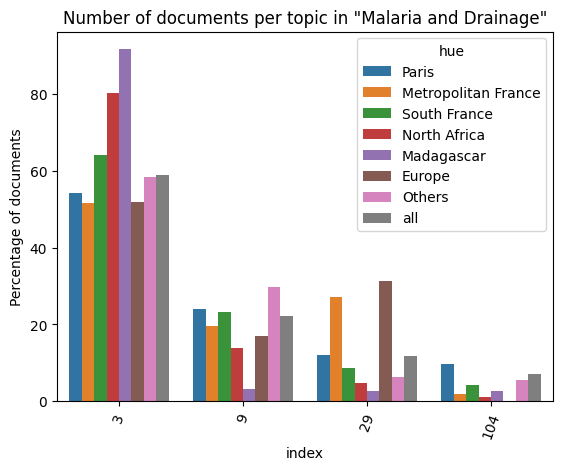
\includegraphics[width=0.5\linewidth]{Images/Figures/dist_malaria_place.png}
    \caption{Bar plot displaying the percentage of topics per place of publication, within the documents containing at least once the meta-topic "Malaria and Drainage".}
    \label{fig:dist_malaria_place}
\end{figure}

Another interesting result from Figure \ref{fig:dist_malaria_place} is the distributions of topic 29, which needs explaining. While at a first glance topic 29 would be linked with "Geography" instead of "Malaria and Drainage", with words such as "Rome", "campagne", "italien", it actually represents a specific policy of eucalyptus plantations in the Roman Campagna, to drain the marshes and purify the air, led by the Trappist abbey of Tre Fontaine\footnote{\cite{noauthor_eucalyptus_1883}}. Thus, it is not surprising to see that around 30\% of documents published in Europe touch on this issue. However, metropolitan France also has around 25\% of documents touching on this topic, which is surprising, as the rest of France does not. By looking over the documents, we see that 26\% of all contexts in which topic 29 appears are in the book "Culture de l'eucalyptus à St-Paul-Trois-Fontaines (près Rome)", published in 1882 in Landerneau. As the title suggest, it speaks about the previously mentioned campaign of eucalyptus plantation around Rome, and the benefits of draining the marshes. While this monograph only does not explain the 10\% difference between the general corpus and metropolitan France, it is a way to understand why this particular incident is talked about in the region, especially since the sample size is relatively small (only 36 documents in metropolitan France mention topic 29). Moreover, most documents in the region speaking about this topic are religious in nature, such as "La Semaine religieuse du diocèse de Rouen", which comes from the fact that it was clergymen that started these eucalyptus plantations, and thus their feat is relayed through the ecclesiastic press. 

Then, we can see what other topics are associated with the meta-topic. By using the graph of co-occurrence, we can then see which topics appear the most next to the topics linked with drainage. Taking topic 3, as it is the biggest topic, it appears most frequently next to topic 7, 14 and 79. The first two are associated with botanical properties of eucalyptus. The first describes its physical properties such as height and circumference, while the second describes its temperature requirements. These appear often together ($\sim$200 documents), as either there is a need to study the plant before committing to these drainage projects, or to introduce what kind of tree is already being used in the new plantations to the public. Probably both are true, as we see that while 60\% of these co-occurrence happen in scientific publications (monographs or scientific press), there are still 31\% that appear in the generalist press. Lastly, we can look at topic 79, which is linked with the Mediterranean, notably the French Mediterranean coast. This shows where these projects are being established, again reinforcing the fact that it is in the Mediterranean basin that eucalyptus are massively being planted. 

Finally, we can look at these topics over time (Figure \ref{fig:dist_malaria_year}). Mentions of drainage and malaria (topics 3 and 9) start appearing in 1870, with a peak in 1875-76. This time frame is linked with several key events, such as the general start of the implementation of large eucalyptus plantations or the end of the Algerian outbreak of the disease. With some decline both topics stay present throughout the years until the start of the war. More over, the curve of the two topics seems to follow similar trends, showing that they are often used together. As regarding topic 29, we do see an increase in 1875-76, followed by a progressive decline. This rise is probably linked with the first results of the Trappist's plantations, starting in 1869, with a gradual decrease, the further from the initial results.

\begin{figure}[H]
    \centering
    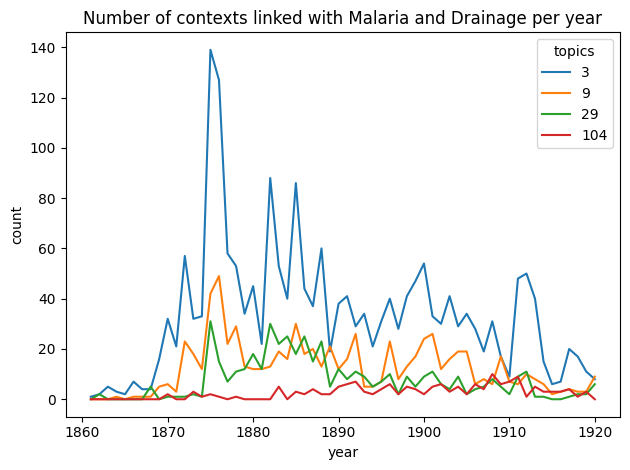
\includegraphics[width=0.5\linewidth]{Images/Figures/dist_malaria_year.png}
    \caption{Line plot displaying the yearly number of contexts linked with topics 3, 9, 29 and 104.}
    \label{fig:dist_malaria_year}
\end{figure}

In conclusion, while a key reason for the development of eucalyptus plantations, the topic of drainage and malaria is not the most discussed in the corpus. However, we do find that it is not insignificant and it is constantly found in all places of publication, with two main topics (3 and 9) in the biggest topics found in the corpus. This theme starts to appear around 1870, when the first large plantations used to sanitize marshes start to appear. Moreover, the model finds a specific event, with the plantation of eucalyptus by Trappist monks in the marshes of Rome. Being linked with the church, it explains why this Italian issue is talked in metropolitan France, though several church journals pushing the virtues of the plant. Moreover, the regular co-occurrence with topics describing the trees botanical characteristics show the way the drainage process is discussed, and which regions are part of the process.
